\documentclass[11pt,a4paper]{ctexart}
% Shared preamble for the assignment reports. Use with:
%   \documentclass[11pt,a4paper]{ctexart}  (XeLaTeX)
%   % Shared preamble for the assignment reports. Use with:
%   \documentclass[11pt,a4paper]{ctexart}  (XeLaTeX)
%   % Shared preamble for the assignment reports. Use with:
%   \documentclass[11pt,a4paper]{ctexart}  (XeLaTeX)
%   \input{../common/preamble.tex}
\usepackage[margin=2.3cm]{geometry}
\setmainfont{texgyretermes}[Extension=.otf,UprightFont=*-regular,BoldFont=*-bold,ItalicFont=*-italic,BoldItalicFont=*-bolditalic]
\setsansfont{texgyreheros}[Extension=.otf,UprightFont=*-regular,BoldFont=*-bold,ItalicFont=*-italic,BoldItalicFont=*-bolditalic]
\setmonofont{texgyrecursor}[Extension=.otf,UprightFont=*-regular,BoldFont=*-bold,ItalicFont=*-italic,BoldItalicFont=*-bolditalic]
\usepackage{amsmath,amssymb,mathtools,bm}
\usepackage{graphicx}
\usepackage{booktabs,multirow,makecell,array,tabularx}
\usepackage[table]{xcolor}
\usepackage[most]{tcolorbox}
\usepackage{enumitem}
\usepackage{listings}
\usepackage{subcaption}
\usepackage{siunitx}
\usepackage[hidelinks]{hyperref}
\usepackage[nameinlink,noabbrev]{cleveref}
\usepackage{float}

\setlength{\emergencystretch}{3em}
\linespread{1.15}
\setlist{leftmargin=*,itemsep=2pt,topsep=3pt}
\graphicspath{{figures/}}

\crefname{figure}{图}{图}
\crefname{table}{表}{表}
\crefname{section}{第}{第}
\creflabelformat{section}{#2#1#3 节}
\crefname{equation}{式}{式}
\crefformat{equation}{式~(#2#1#3)}

\lstset{basicstyle=\ttfamily\footnotesize,columns=fullflexible,breaklines=true,frame=single,
  framerule=0.3pt,rulecolor=\color{black!40},backgroundcolor=\color{black!3},
  keywordstyle=\color{blue!60!black}\bfseries,commentstyle=\color{green!40!black},
  numbers=left,numberstyle=\tiny\color{black!50},xleftmargin=1.5em}

% Interview boxes: question, model answer, common wrong answer.
\newtcolorbox{iqbox}[1]{enhanced,breakable,colback=blue!3,colframe=blue!45!black,boxrule=0.5pt,arc=1.5pt,
  left=4pt,right=4pt,top=3pt,bottom=3pt,fonttitle=\bfseries\small,title={面试追问：#1}}
\newtcolorbox{findingbox}[1][]{enhanced,breakable,colback=green!3,colframe=green!40!black,boxrule=0.5pt,arc=1.5pt,
  left=4pt,right=4pt,top=3pt,bottom=3pt,fonttitle=\bfseries\small,title={结论#1}}
\newtcolorbox{caveatbox}{enhanced,breakable,colback=orange!4,colframe=orange!60!black,boxrule=0.5pt,arc=1.5pt,
  left=4pt,right=4pt,top=3pt,bottom=3pt,fonttitle=\bfseries\small,title={不能推出的结论}}

\newcommand{\authorline}{ShaneLiu04\thanks{GitHub: \url{https://github.com/ShaneLiu04}。代码与原始指标见 edge-deploy 仓库各 lab 的 \texttt{artifacts/raw/}。本文基于公开课程材料独立完成，与课程团队无隶属关系。}}

\usepackage[margin=2.3cm]{geometry}
\setmainfont{texgyretermes}[Extension=.otf,UprightFont=*-regular,BoldFont=*-bold,ItalicFont=*-italic,BoldItalicFont=*-bolditalic]
\setsansfont{texgyreheros}[Extension=.otf,UprightFont=*-regular,BoldFont=*-bold,ItalicFont=*-italic,BoldItalicFont=*-bolditalic]
\setmonofont{texgyrecursor}[Extension=.otf,UprightFont=*-regular,BoldFont=*-bold,ItalicFont=*-italic,BoldItalicFont=*-bolditalic]
\usepackage{amsmath,amssymb,mathtools,bm}
\usepackage{graphicx}
\usepackage{booktabs,multirow,makecell,array,tabularx}
\usepackage[table]{xcolor}
\usepackage[most]{tcolorbox}
\usepackage{enumitem}
\usepackage{listings}
\usepackage{subcaption}
\usepackage{siunitx}
\usepackage[hidelinks]{hyperref}
\usepackage[nameinlink,noabbrev]{cleveref}
\usepackage{float}

\setlength{\emergencystretch}{3em}
\linespread{1.15}
\setlist{leftmargin=*,itemsep=2pt,topsep=3pt}
\graphicspath{{figures/}}

\crefname{figure}{图}{图}
\crefname{table}{表}{表}
\crefname{section}{第}{第}
\creflabelformat{section}{#2#1#3 节}
\crefname{equation}{式}{式}
\crefformat{equation}{式~(#2#1#3)}

\lstset{basicstyle=\ttfamily\footnotesize,columns=fullflexible,breaklines=true,frame=single,
  framerule=0.3pt,rulecolor=\color{black!40},backgroundcolor=\color{black!3},
  keywordstyle=\color{blue!60!black}\bfseries,commentstyle=\color{green!40!black},
  numbers=left,numberstyle=\tiny\color{black!50},xleftmargin=1.5em}

% Interview boxes: question, model answer, common wrong answer.
\newtcolorbox{iqbox}[1]{enhanced,breakable,colback=blue!3,colframe=blue!45!black,boxrule=0.5pt,arc=1.5pt,
  left=4pt,right=4pt,top=3pt,bottom=3pt,fonttitle=\bfseries\small,title={面试追问：#1}}
\newtcolorbox{findingbox}[1][]{enhanced,breakable,colback=green!3,colframe=green!40!black,boxrule=0.5pt,arc=1.5pt,
  left=4pt,right=4pt,top=3pt,bottom=3pt,fonttitle=\bfseries\small,title={结论#1}}
\newtcolorbox{caveatbox}{enhanced,breakable,colback=orange!4,colframe=orange!60!black,boxrule=0.5pt,arc=1.5pt,
  left=4pt,right=4pt,top=3pt,bottom=3pt,fonttitle=\bfseries\small,title={不能推出的结论}}

\newcommand{\authorline}{ShaneLiu04\thanks{GitHub: \url{https://github.com/ShaneLiu04}。代码与原始指标见 edge-deploy 仓库各 lab 的 \texttt{artifacts/raw/}。本文基于公开课程材料独立完成，与课程团队无隶属关系。}}

\usepackage[margin=2.3cm]{geometry}
\setmainfont{texgyretermes}[Extension=.otf,UprightFont=*-regular,BoldFont=*-bold,ItalicFont=*-italic,BoldItalicFont=*-bolditalic]
\setsansfont{texgyreheros}[Extension=.otf,UprightFont=*-regular,BoldFont=*-bold,ItalicFont=*-italic,BoldItalicFont=*-bolditalic]
\setmonofont{texgyrecursor}[Extension=.otf,UprightFont=*-regular,BoldFont=*-bold,ItalicFont=*-italic,BoldItalicFont=*-bolditalic]
\usepackage{amsmath,amssymb,mathtools,bm}
\usepackage{graphicx}
\usepackage{booktabs,multirow,makecell,array,tabularx}
\usepackage[table]{xcolor}
\usepackage[most]{tcolorbox}
\usepackage{enumitem}
\usepackage{listings}
\usepackage{subcaption}
\usepackage{siunitx}
\usepackage[hidelinks]{hyperref}
\usepackage[nameinlink,noabbrev]{cleveref}
\usepackage{float}

\setlength{\emergencystretch}{3em}
\linespread{1.15}
\setlist{leftmargin=*,itemsep=2pt,topsep=3pt}
\graphicspath{{figures/}}

\crefname{figure}{图}{图}
\crefname{table}{表}{表}
\crefname{section}{第}{第}
\creflabelformat{section}{#2#1#3 节}
\crefname{equation}{式}{式}
\crefformat{equation}{式~(#2#1#3)}

\lstset{basicstyle=\ttfamily\footnotesize,columns=fullflexible,breaklines=true,frame=single,
  framerule=0.3pt,rulecolor=\color{black!40},backgroundcolor=\color{black!3},
  keywordstyle=\color{blue!60!black}\bfseries,commentstyle=\color{green!40!black},
  numbers=left,numberstyle=\tiny\color{black!50},xleftmargin=1.5em}

% Interview boxes: question, model answer, common wrong answer.
\newtcolorbox{iqbox}[1]{enhanced,breakable,colback=blue!3,colframe=blue!45!black,boxrule=0.5pt,arc=1.5pt,
  left=4pt,right=4pt,top=3pt,bottom=3pt,fonttitle=\bfseries\small,title={面试追问：#1}}
\newtcolorbox{findingbox}[1][]{enhanced,breakable,colback=green!3,colframe=green!40!black,boxrule=0.5pt,arc=1.5pt,
  left=4pt,right=4pt,top=3pt,bottom=3pt,fonttitle=\bfseries\small,title={结论#1}}
\newtcolorbox{caveatbox}{enhanced,breakable,colback=orange!4,colframe=orange!60!black,boxrule=0.5pt,arc=1.5pt,
  left=4pt,right=4pt,top=3pt,bottom=3pt,fonttitle=\bfseries\small,title={不能推出的结论}}

\newcommand{\authorline}{ShaneLiu04\thanks{GitHub: \url{https://github.com/ShaneLiu04}。代码与原始指标见 edge-deploy 仓库各 lab 的 \texttt{artifacts/raw/}。本文基于公开课程材料独立完成，与课程团队无隶属关系。}}

\graphicspath{{../../solutions/mit6.5940/tinyengine-memory/artifacts/figures/}}

\title{MIT 6.5940 TinyEngine / MCUNetV2 实验报告：\\激活峰值下界、arena 规划、原地 depthwise 与按 patch 推理}
\author{\authorline}
\date{2026 年 11 月}

% Equation numbers follow interview/FORMULAS.md (M04 = E10--E14).
\renewcommand{\theequation}{E\arabic{equation}}
\setcounter{equation}{9}

\begin{document}
\maketitle

\begin{abstract}
MIT 6.5940（TinyML and Efficient Deep Learning）的 TinyEngine 与 MCUNet / MCUNetV2 两讲要解决的是同一个问题：
MCU 上权重放 Flash，激活放几百 KB 的 SRAM，先撞墙的是\emph{激活峰值}而不是参数量。
本报告在 PyTorch 模型上用 \texttt{torch.fx} trace 出每个 int8 激活缓冲的生死区间，把内存规划写成一维装箱，
比较每块独占、first-fit、按大小降序贪心（TFLite Micro \texttt{GreedyMemoryPlanner} 的顺序）三种放置与存活下界，
再实现 TinyEngine 的原地 depthwise 和 MCUNetV2 的按 patch 推理，量化“峰值换重算”的权衡。
模型是本仓库 lab2 的 micro-MobileNetV2（32/64/96 分辨率）与 torchvision MobileNetV2 宽度 0.35 / 1.0（96/128/160/224），共 11 个配置；纯 Python，不需要硬件，全部实验约 10 秒。

主要结论：
（a）按大小降序贪心在全部 11 个配置上\emph{正好等于}存活下界（碎片率 0）；按出生顺序 first-fit 在 8 个 MobileNetV2 配置上都多 13.3\%，
    在线性链结构的 micro 网络上为 0；每块独占是下界的 3.58--4.69 倍；
（b）原地 depthwise 让 MobileNetV2 峰值再降 6.7\%（1.0@224：1,505,280 → 1,404,928 B），micro 网络降 30.8\%；
    整网峰值只能降到“第二高点”，而且原地之后 micro 网络上贪心不再贴住新下界（55,296 对 49,152 B，多 12.5\%）；
（c）按 patch 推理：MBv2-0.35@160 前 4 个 block 切 3×3，峰值 384,000 → 102,400 B（3.75 倍），整网 MACs 多 27\%；
    1.0@224 切 2×2，1,505,280 → 566,784 B，整网 MACs 只多 7.7\%；
（d）切得越深越细，重算越贵：0.35@160 切 8 个 block、4×4 时整网 MACs 是 4.21 倍，峰值却只降到 177,360 B，比切 4 个 block 的 102,400 B 还高——
    halo 随层深线性外扩，重算按 $p^2$ 增长，而峰值一旦转移到 cut 之后的层就不再下降。
\end{abstract}

\tableofcontents
\newpage

\section{这个实验要回答什么}

\subsection{课程背景}
MIT 6.5940 Fall 2024 的《TinyEngine~\cite{mcunet} and Parallel Processing》与《MCUNet / MCUNetV2~\cite{mcunetv2}》两讲给出一个反直觉的事实：
一块 Cortex-M7 的 STM32F746 有 320 KB SRAM、1 MB Flash，MobileNetV2~\cite{mobilenetv2}-1.0 的 int8 权重 3.6 MB 已经放不进 Flash，
但即使换成更小的网络，先放不下的往往是激活——SRAM 要同时容纳“当前算子的输入 + 输出 + 仍然存活等着被残差读取的张量”。
TFLite Micro（TFLM）把所有激活放在一块用户预先分配的 \emph{arena} 里，编译期用 \texttt{GreedyMemoryPlanner} 给每个张量一个偏移；
TinyEngine 在此基础上做原地 depthwise；MCUNetV2 进一步把前几层按空间 patch 执行，让最大的激活永远不整块存在。

\subsection{要回答的四个问题}
\begin{enumerate}
  \item 给定一张推理图，最少需要多少 SRAM？——存活字节的时间最大值（下界，E10）。
  \item 现成的规划器离下界多远？——碎片率（E11），以及放置顺序如何制造碎片。
  \item 下界本身能不能压？——原地 depthwise 改变“同时存活”的定义；它能省多少，取决于峰值转移到哪里。
  \item 用算力换内存划算到什么程度？——patch 推理的 halo 回推（E12）、重算比例（E13）、峰值组成（E14），以及“stage 口径”与“整网口径”的区别。
\end{enumerate}

\subsection{和原课程的差异}
TinyEngine 生成 C 代码并在 MCU 上实测延迟与内存；本实验只做规划与字节账，不生成代码、不测延迟。
存活期由 \texttt{torch.fx} trace 加一次 shape 传播得到，BN、ReLU 融合后视为别名（不分配新内存），残差的输入一直存活到相加。
GPU 训练侧的同一问题（激活重计算~\cite{chen2016}、显存规划）见姊妹仓库 mlsys-infra 的 M14，本报告\cref{sec:discussion}做了对照。

\section{设置}

\subsection{模型与配置}

\begin{table}[H]
\centering\small
\caption{模型与分辨率（int8 激活，batch 1，16 字节对齐）}\label{tab:models}
\begin{tabularx}{\linewidth}{l r r r >{\raggedright\arraybackslash}X}
\toprule
模型 & 分辨率 & 缓冲数 & int8 权重 B & 说明 \\
\midrule
micro-mbv2（本仓库） & 32 / 64 / 96 & 32 & 231,656 & lab2 的 CIFAR-10 网络，线性链 + 残差 \\
MBv2 宽度 0.35 & 96 / 128 / 160 / 224 & 65 & 1,722,368 & torchvision，\texttt{width\_mult=0.35}，随机权重 \\
MBv2 宽度 1.0 & 96 / 128 / 160 / 224 & 65 & 3,610,208 & torchvision，\texttt{width\_mult=1.0}，随机权重 \\
\bottomrule
\end{tabularx}
\end{table}

内存规划只依赖张量形状与图结构，与权重数值无关，所以 torchvision 模型用随机权重即可。
“int8 权重 B”是 \texttt{flash\_bytes}：二维以上参数按 1 字节、一维参数（偏置等）按 4 字节计，用来说明 Flash 侧是否放得下。

\subsection{MCU 预算是参数，不是测量}
SRAM 预算取自仓库的设备表 \texttt{edge\_harness/devices.py}（STM32F746 那一项是脚本里直接写的 $320\times1024$ 字节，MCUNet 论文报告的板子）。
它们只是用来画线和判定“放不放得下”的\emph{参数}，本实验没有在任何一块板子上运行。

\begin{table}[H]
\centering\small
\caption{MCU 预算（字节按 1 KB = 1024 B）}\label{tab:budgets}
\begin{tabular}{llrr}
\toprule
设备 & 核心 & SRAM & Flash \\
\midrule
Nordic nRF52840 & Cortex-M4F，64 MHz & 256 KB = 262,144 B & 1 MB \\
STMicro STM32F746 & Cortex-M7 & 320 KB = 327,680 B & — \\
STMicro STM32H747 & Cortex-M7 + M4，480 MHz & 1 MB = 1,048,576 B & 2 MB \\
\bottomrule
\end{tabular}
\end{table}

\subsection{代码结构}
\begin{table}[H]
\centering\small
\caption{实现映射}\label{tab:code}
\begin{tabularx}{\linewidth}{l >{\raggedright\arraybackslash}X}
\toprule
文件 & 内容 \\
\midrule
\texttt{code/memplan/graph.py} & \texttt{trace}：fx 图 → 缓冲列表（大小、出生、死亡），处理融合别名与残差；\texttt{inplace\_depthwise}；\texttt{live\_profile} \\
\texttt{code/memplan/planners.py} & \texttt{lower\_bound}、\texttt{naive}、\texttt{first\_fit}、\texttt{greedy\_by\_size}、\texttt{arena\_size}、\texttt{validate} \\
\texttt{code/memplan/patch.py} & \texttt{input\_extent}（halo 回推）、\texttt{macs}、\texttt{patch\_plan}（峰值与重算） \\
\texttt{scripts/run\_experiments.py} & \texttt{step\_planners}、\texttt{step\_profile}、\texttt{step\_patch}、\texttt{summarize} \\
\texttt{tests/test\_memplan.py} & 9 个测试：下界、碎片反例、重叠检测、融合与残差、原地 dw、halo、patch 权衡 \\
\bottomrule
\end{tabularx}
\end{table}

\section{方法与推导}\label{sec:method}

\subsection{张量的生死与别名}
\texttt{trace} 按 fx 图的拓扑顺序给每个产生新缓冲的节点一个步号 $t$。缓冲 $i$ 的出生时刻 $b_i$ 是写它的算子的步号，死亡时刻 $d_i$ 是最后一个读它的算子的步号；
图输入从第 0 步存活，图输出活到最后一步之后。下面三类节点不分配新内存，而是别名到它的输入缓冲：
\begin{itemize}
  \item BN：部署前已折进卷积（lab2 的 BN 折叠）；
  \item ReLU / ReLU6 / Hardswish：在 int8 kernel 里就是 requant 之后的 clamp；
  \item flatten / view / reshape / contiguous / Identity / Dropout：只改形状或推理时为恒等。
\end{itemize}
测试 \texttt{test\_trace\_fuses\_bn\_relu\_and\_keeps\_residual\_input\_alive} 检查：缓冲生产者里没有 BN / ReLU；每个残差 add 的两个输入都活到 add 的步号。
如果忘记别名，把 BN、ReLU 各算一块输出，MobileNetV2 的峰值会被虚增一倍以上——这是 M04 笔记列出的头号易错点。

\subsection{峰值下界}
在任意时刻 $t$，所有存活缓冲必须占据互不重叠的地址，因此 arena 至少要有
\begin{equation}
  L = \max_t \sum_{i:\, b_i \le t \le d_i} s_i , \label{eq:e10}
\end{equation}
其中 $s_i$ 是缓冲 $i$ 的字节数（向上对齐到 16）。存活集合只在某个缓冲出生时变大，死亡时只会变小，所以最大值一定在某个出生时刻取到；
\texttt{lower\_bound} 只扫描 $\{b_i\}$，复杂度 $O(n^2)$，对几十个缓冲足够。测试 \texttt{test\_planners\_valid\_and\_ordered\_on\_mobilenet} 同时验证 \texttt{max(live\_profile)} 与 $L$ 相等。

\subsection{四种“规划器”}
一个放置方案给每个缓冲一个偏移 $o_i$，要求存活期相交的两块地址不重叠；arena 大小与碎片率为
\begin{equation}
  A = \max_i (o_i + s_i) \;\ge\; L, \qquad \text{碎片率} = A / L - 1 . \label{eq:e11}
\end{equation}
本实验比较四个量：
\begin{description}[leftmargin=1.5em]
  \item[下界 \texttt{lower\_bound}] 即 \cref{eq:e10}，不是规划器而是任何规划器都打不破的参照。
  \item[每块独占 \texttt{naive}] 偏移累加，$A=\sum_i s_i$。相当于不做内存复用。
  \item[first-fit] 按出生顺序（同时出生的先放大的）逐块放置，每块放在与所有已放置、存活期相交的块都不冲突的最低偏移。
  \item[按大小贪心 \texttt{greedy\_by\_size}] 同样的“最低可行偏移”规则，但按大小降序（同样大小按出生顺序）放置。这是 TFLM \texttt{GreedyMemoryPlanner} 的顺序。
\end{description}
两种贪心共用 \texttt{\_place}：对当前块，把与它存活期相交的已放置块的地址区间排序，从 0 开始找第一个放得下的空隙。
\texttt{validate} 对所有存活期相交的块对检查地址不重叠，每个实验配置的每个方案都过了这道检查。

\subsection{碎片反例：放置顺序决定碎片}
\texttt{tests/test\_memplan.py} 里的反例有四块缓冲（大小，出生，死亡）：
small（10, 0, 4）、big1（100, 1, 2）、mid（60, 0, 0）、big2（100, 3, 4）。
时刻 0 存活 small + mid = 70，时刻 1--2 存活 small + big1 = 110，时刻 3--4 存活 small + big2 = 110，下界 $L=110$。
用 \texttt{planners.py} 在这组输入上算得的放置如\cref{tab:frag}。

\begin{table}[H]
\centering\small
\caption{碎片反例：两种放置顺序（由 \texttt{planners.py} 在测试输入上算出）}\label{tab:frag}
\begin{tabular}{lllllr}
\toprule
规划器 & mid & small & big1 & big2 & arena \\
\midrule
first-fit（出生顺序） & 0 & 60 & 70 & 70 & 170 \\
按大小贪心 & 0 & 100 & 0 & 0 & 110 \\
每块独占 & 110 & 0 & 10 & 170 & 270 \\
\midrule
下界 $L$ & \multicolumn{4}{l}{} & 110 \\
\bottomrule
\end{tabular}
\end{table}

first-fit 的问题是 \emph{小而长寿}的 small 出生最早，被放在 mid 上方的 60；mid 死后低地址空出一个 60 字节的洞，但两个 100 字节的大块都塞不进去，只能叠在 small 上方，arena 170（碎片率 54.5\%）。
按大小贪心先让 big1、big2 占住 0 偏移（它们存活期不相交，可以共用），mid 也放在 0（与两个大块都不同时存活），最后 small 填到 100，正好等于下界。

但按大小贪心不是最优算法。M04 笔记的另一个例子：A（3, 0, 0）、B（3, 0, 1）、C（2, 1, 1）、D（2, 1, 1），下界 7；
用同一份代码算，first-fit 与按大小贪心给出\emph{同一个}放置（A@0、B@3、C@0、D@6），arena 都是 8，而 B@0、A@3、C@3、D@5 可以做到 7。
大小相同时按出生顺序打破平局，让 A 占住低地址、把 B 卡在中间。带大小的动态存储分配是 NP-hard 问题，贪心在 MobileNet 这一类近似链式的图上贴住下界是经验规律，不是定理。

\subsection{原地 depthwise}\label{sec:inplace-method}
depthwise 卷积的输出通道 $c$ 只依赖输入通道 $c$。TinyEngine 按通道顺序计算，用一个“一个输入通道大小”的临时缓冲存当前通道结果，算完写回输入的位置，
于是输入与输出共享一块 $\max(s_\text{in}, s_\text{out})$ 的内存，外加一个 $H\times W$ 的 scratch。\texttt{inplace\_depthwise} 的合并条件有两个：
\begin{enumerate}
  \item 逐通道依赖：\texttt{groups == in\_channels == out\_channels}；
  \item 输入在 depthwise 之后不再被读（\texttt{src.death == t.birth}），即没有残差从 depthwise 的输入引出。
\end{enumerate}
stride 2 同样成立，因为一个通道的输出先整块写进 scratch 再拷回，不存在行内覆盖顺序的问题。普通 3×3 卷积不能原地：输出位置 $(y,x)$ 依赖输入 $(y\pm1, x\pm1)$ 的\emph{全部}通道，覆盖后邻居读到的是新值。

一个倒残差块 expand(1×1) → dw(3×3) → project(1×1) 在 dw 处不原地时同时存活 expand 输出与 dw 输出；原地后只剩 $\max$ 加一个通道。
以 MBv2-1.0@224 为例（M04 笔记的白板估算，与实测下界逐字节一致）：
\begin{align*}
  \text{dw 处（不原地）}&: 112\times112\times96 + 56\times56\times96 = 1{,}204{,}224 + 301{,}056 = 1{,}505{,}280 \text{ B} \quad(= L)\\
  \text{dw 处（原地）}&: 1{,}204{,}224 + 112\times112 = 1{,}216{,}768 \text{ B}\\
  \text{expand 处}&: 112\times112\times16 + 1{,}204{,}224 = 200{,}704 + 1{,}204{,}224 = 1{,}404{,}928 \text{ B} \quad(= L_\text{原地})
\end{align*}
dw 处省下了 288,512 B，但整网峰值随即转移到同一个 block 的 expand 处，只降 100,352 B（6.7\%）。
所以“原地省多少”不能只看单层，要看第二高点在哪。

\subsection{按 patch 推理：halo 回推、重算与峰值}
MCUNetV2 把 \texttt{features[:k]}（cut = $k$）这一段按空间 tile 执行：cut 处输出 $H_\text{out}\times H_\text{out}$ 切成 $p\times p$ 块，
每块输出宽 $t_\text{out}=\lceil H_\text{out}/p\rceil$。为算出这一块，要从 cut 处逐层往输入回推所需的区域：
\begin{equation}
  w_\text{in} = (w_\text{out}-1)\cdot \text{stride} + \text{kernel} , \label{eq:e12}
\end{equation}
\texttt{input\_extent} 对 stage 里每个卷积按逆序应用 \cref{eq:e12}（1×1、stride 1 的卷积不改变范围），结果截断到全图分辨率。
测试锚点：$[(3,2),(3,1)]$ 从输出 4 回推得 $(4-1)\cdot1+3=6$，再 $(6-1)\cdot2+3=13$。

相邻 tile 的 halo 被重复计算，重算比例有两种口径：
\begin{equation}
  \text{stage 开销} = \frac{p^2\cdot \mathrm{MACs}(\text{tile}_\text{in})}{\mathrm{MACs}(\text{全图})}, \qquad
  \text{整网开销} = \frac{p^2\cdot \mathrm{MACs}(\text{tile}_\text{in}) + \mathrm{MACs}(\text{其余层})}{\mathrm{MACs}(\text{整网})} . \label{eq:e13}
\end{equation}
记 stage 占整网 MACs 的比例为 $f$，则 整网开销 $= 1 + (\text{stage 开销}-1)\cdot f$。论文和博客常报 stage 口径；部署关心的是整网口径。

patch 执行时 cut 处的完整输出缓冲必须整块存在（各 tile 写进去），stage 内只需容纳一个 tile 的中间激活，峰值为
\begin{equation}
  \text{peak} = \max\bigl(\underbrace{s_\text{stage\_out} + \mathrm{peak}(\text{单 tile 跑 stage})}_{\text{patch\_stage\_peak}},\;
  \underbrace{\mathrm{peak}(\text{cut 之后的层})}_{\text{rest\_peak}}\bigr) . \label{eq:e14}
\end{equation}
两项都用按大小贪心规划（\texttt{peak}），不叠加原地 depthwise。$p=1$ 时退化为整图执行。

\begin{iqbox}{给你一张推理图，最少要多少 SRAM？TFLM 的 arena 大小怎么定？}
先从图里算每个激活缓冲的生死区间，BN、ReLU、flatten 这类融合后不分配的节点要当作别名，然后取 \cref{eq:e10} 的存活峰值，这是任何规划都打不破的下界。
TFLM 编译期跑一遍 \texttt{GreedyMemoryPlanner}（按大小降序放置）得到高水位 $A$，再加上算子 scratch（如 im2col）和持久缓冲、interpreter 自身开销。
本实验的 11 个配置上贪心的 $A$ 正好等于 $L$，所以“激活部分”的 arena 就是下界；实践中先给一个大 arena，读 \texttt{arena\_used\_bytes()} 再收紧。
常见错答是“把所有激活加起来”——那是每块独占，是下界的 3.6--4.7 倍。
\end{iqbox}

\section{结果一：规划器与下界}\label{sec:planners}

\begin{table}[H]
\centering\small
\caption{规划器 arena 大小（字节，int8 激活，batch 1；完整 11 行，\texttt{planners.csv}）}\label{tab:planners}
\begin{tabular}{lrrrrrr}
\toprule
模型@分辨率 & 下界 $L$ & 每块独占 & 独占 / $L$ & first-fit & 碎片率 & 按大小贪心 \\
\midrule
micro@32 & 79,872 & 286,480 & 3.59 & 79,872 & 0 & 79,872 \\
micro@64 & 319,488 & 1,145,104 & 3.58 & 319,488 & 0 & 319,488 \\
micro@96 & 718,848 & 2,576,144 & 3.58 & 718,848 & 0 & 718,848 \\
\midrule
MBv2-0.35@96 & 138,240 & 570,912 & 4.13 & 156,672 & 13.3\% & 138,240 \\
MBv2-0.35@128 & 245,760 & 1,013,104 & 4.12 & 278,528 & 13.3\% & 245,760 \\
MBv2-0.35@160 & 384,000 & 1,581,728 & 4.12 & 435,200 & 13.3\% & 384,000 \\
MBv2-0.35@224 & 752,640 & 3,097,952 & 4.12 & 852,992 & 13.3\% & 752,640 \\
\midrule
MBv2-1.0@96 & 276,480 & 1,296,272 & 4.69 & 313,344 & 13.3\% & 276,480 \\
MBv2-1.0@128 & 491,520 & 2,302,704 & 4.68 & 557,056 & 13.3\% & 491,520 \\
MBv2-1.0@160 & 768,000 & 3,596,688 & 4.68 & 870,400 & 13.3\% & 768,000 \\
MBv2-1.0@224 & 1,505,280 & 7,047,312 & 4.68 & 1,705,984 & 13.3\% & 1,505,280 \\
\bottomrule
\end{tabular}
\end{table}

\Cref{tab:planners}有三个规律。

\textbf{按大小贪心 11/11 等于下界。}\texttt{greedy\_gap} 一列全部为 0。MobileNet 一类网络近似链式，存活期是一串短区间，大块之间很少“错位重叠”：
大块先放在 0 偏移，小块只需避开同时存活的大块，高水位由最大的那一对相邻激活决定——而这正是下界取到的位置。

\textbf{first-fit 的碎片率在每个 MBv2 配置上都是 13.3\%，与宽度、分辨率无关。}
所有张量大小都随分辨率平方缩放、随宽度近似线性缩放，同一个 block 结构在每个配置上制造出比例相同的洞（$435{,}200/384{,}000 = 1{,}705{,}984/1{,}505{,}280 = 1.133$）。
来源在 MobileNetV2 前几层：一个大张量先放在低地址，之后同样大小的张量只能放在它上面。micro 网络是线性链、没有这种交错，所以 first-fit 也是最优。

\textbf{每块独占是下界的 3.58--4.69 倍。}这一比值也几乎不随分辨率变化，只随结构变化：micro 约 3.6，0.35 宽约 4.1，1.0 宽约 4.7。
MBv2 有 65 个缓冲而 micro 只有 32 个，缓冲越多、寿命越短，复用的收益越大。

\begin{figure}[H]
\centering
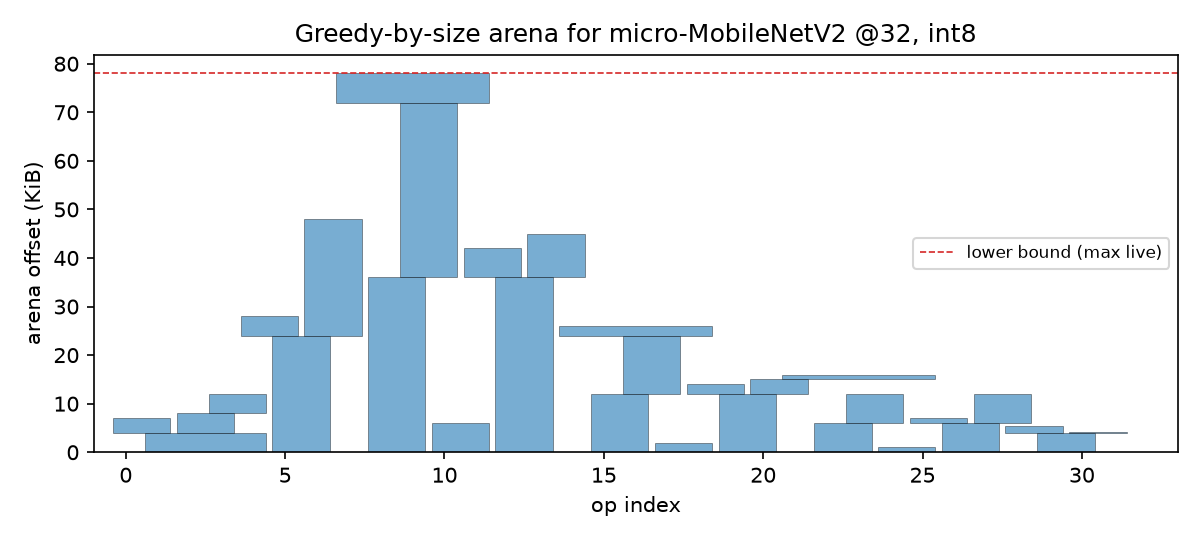
\includegraphics[width=0.95\linewidth]{arena_layout.png}
\caption{micro-MobileNetV2@32 的按大小贪心 arena：每个矩形是一个 int8 缓冲，横向跨度是存活期（op 序号），纵向是偏移（KiB）；红色虚线是存活下界 $L=79{,}872$ B（78 KiB）。}\label{fig:arena}
\end{figure}

\Cref{fig:arena}把规划结果画成“时间 × 地址”平面。读法：任一竖直线穿过的矩形就是那一时刻同时存活的缓冲，它们必须在纵向上互不重叠。
最高的矩形堆叠出现在第 8--11 步附近，顶端正好贴住红线——这就是下界取到的时刻，也是按大小贪心的高水位，二者相等说明这一点上没有任何浪费。
其余时刻纵向都有大块空白，但那些空白不影响 arena 大小：arena 由最高的一列决定，其他列的空隙是“免费的”。
还能看到按大小贪心的典型形状：最大的几块（三十多 KiB 高的那几列）都从 0 偏移或紧贴另一大块放置，小块（只有一两 KiB 高的扁矩形）塞在大块之间的缝里。
图中 32 个缓冲对应\cref{tab:models}的缓冲数。

\begin{findingbox}[：规划器]
按大小降序贪心在 11 个配置上碎片率为 0，按出生顺序 first-fit 在全部 8 个 MobileNetV2 配置上恒为 13.3\%。
对 TFLM 用户的含义是：只要用默认的 \texttt{GreedyMemoryPlanner}，arena 中\emph{激活部分}已经到下界，再想省内存只能改下界本身（原地、patch、改网络），
而不是换规划算法。
\end{findingbox}

\begin{iqbox}{贪心不是最优算法，凭什么说你的 arena 没有浪费？}
不需要证明贪心最优，只需要把它和下界比：\cref{eq:e10} 的 $L$ 是任何放置的下界，\cref{eq:e11} 的 $A$ 是实际高水位，$A=L$ 就说明这张图上没有浪费。
本实验 11 个配置都是 $A=L$。但这是“这类图上碰巧贴住”，不是定理：同一份代码在 A/B/C/D（3、3、2、2）的反例上给出 8，而最优是 7；
带大小的动态存储分配是 NP-hard。所以正确的说法是“先算 $L$ 再谈浪费”，而不是“贪心一定最优”或“贪心一定有浪费”。
\end{iqbox}

\section{结果二：峰值在哪里、原地 depthwise 省多少}\label{sec:profile}

\begin{figure}[H]
\centering
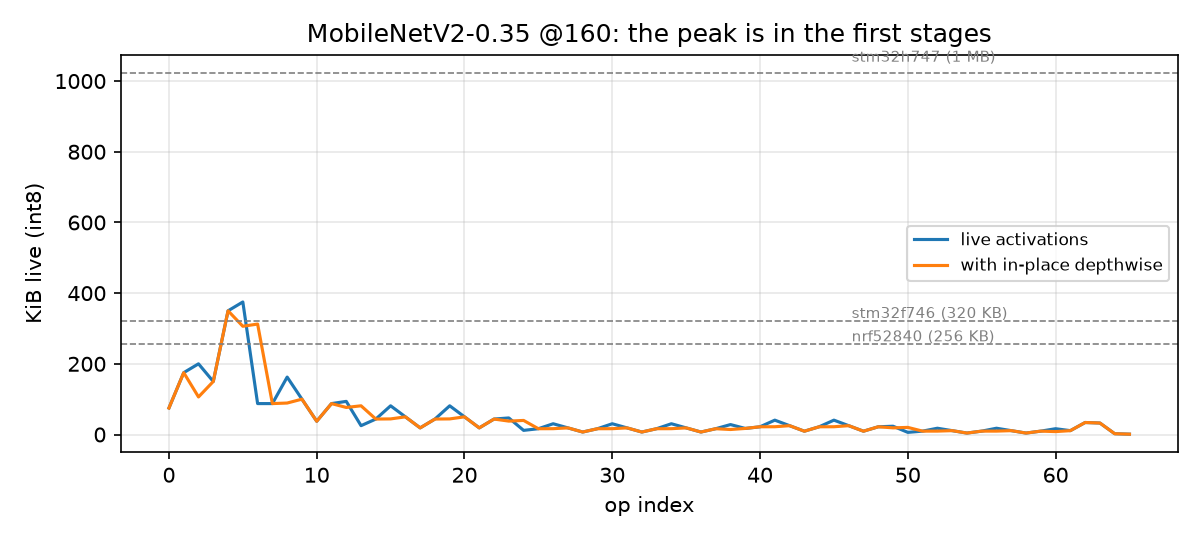
\includegraphics[width=0.95\linewidth]{memory_profile.png}
\caption{MobileNetV2-0.35@160 逐步存活字节（KiB，int8）。蓝线是原始图，橙线是原地 depthwise 之后；灰色虚线是三块 MCU 的 SRAM 预算。}\label{fig:profile}
\end{figure}

\Cref{fig:profile}的读法：横轴是 op 序号（0 是输入），纵轴是那一步同时存活的激活字节。整条曲线的最大值就是\cref{eq:e10}的下界。
峰值集中在前 6 步，第 20 步之后存活量都在 50 KiB 以下，最后几十步只有几 KiB 到几十 KiB。
原因是 MobileNetV2 前几层空间分辨率最高：通道虽少但 $H\times W$ 大，而 expand 比 6 让第二个 block 的中间激活最大；之后每次下采样 $H\times W$ 缩小 4 倍。
三条预算线里，蓝线的峰值高于 nRF52840（256 KB）和 STM32F746（320 KB），只在 STM32H747（1 MB）之下；橙线的峰值仍然高于 320 KB 线。

\begin{table}[H]
\centering\small
\caption{MBv2-0.35@160 前 9 步的存活字节（\texttt{profile\_mbv2\_w035\_160.csv}）与按形状的分解}\label{tab:profile}
\begin{tabularx}{\linewidth}{rrr >{\raggedright\arraybackslash}X}
\toprule
步 & 原始 B & 原地 dw 后 B & 解释（形状由宽度 0.35 推出，与字节数逐一对上） \\
\midrule
0 & 76,800 & 76,800 & 输入 $160\times160\times3$ \\
1 & 179,200 & 179,200 & 输入 + stem 输出 $80\times80\times16=102{,}400$ \\
2 & 204,800 & 108,800 & block 1 的 dw：输入 102,400 + 输出 102,400；原地后 102,400 + 一个通道 $80\times80=6{,}400$ \\
3 & 153,600 & 153,600 & block 1 project \\
4 & 358,400 & 358,400 & block 2 expand：输入 $80\times80\times8=51{,}200$ + 输出 $80\times80\times48=307{,}200$ \\
5 & \textbf{384,000} & 313,600 & block 2 dw（stride 2）：307,200 + 输出 $40\times40\times48=76{,}800$；原地后 307,200 + 6,400 \\
6 & 89,600 & 320,000 & block 2 project：原始 76,800 + 12,800；原地后合并缓冲仍按 307,200 存活 + 12,800 \\
7 & 89,600 & 89,600 & — \\
8 & 166,400 & 91,200 & 下一个 dw，原地同样生效 \\
\bottomrule
\end{tabularx}
\end{table}

\Cref{tab:profile}把曲线前段逐步拆开，几个现象值得注意：
\begin{itemize}
  \item 原始峰值 384,000 B 在第 5 步，即 block 2 的 stride-2 depthwise：expand 输出与 dw 输出同时存活。
  \item 原地 depthwise 把第 2 步从 204,800 压到 108,800、第 5 步从 384,000 压到 313,600，但第 4 步（expand 处）不受影响，于是整网峰值降到第二高点 358,400 B，只省 6.7\%。
  \item \emph{原地也有代价}：第 6 步从 89,600 涨到 320,000。合并后的缓冲大小是 $\max(s_\text{in}, s_\text{out})=307{,}200$，而它要活到 dw 输出的最后一个读者（project）为止；
        原始图里那时只剩 76,800 的 dw 输出。\Cref{fig:profile}里橙线在第 6 步的凸起就是这个。它没有超过第 4 步，所以不影响峰值，但说明原地是“用更长的大块寿命换更少的同时存活块”。
\end{itemize}

\begin{table}[H]
\centering\small
\caption{原地 depthwise 的效果（字节，\texttt{planners.csv}）}\label{tab:inplace}
\begin{tabular}{lrrrrr}
\toprule
模型@分辨率 & 贪心 & 原地 + 贪心 & 原地后下界 & 节省 & 原地后碎片率 \\
\midrule
micro@32 & 79,872 & 55,296 & 49,152 & 30.8\% & 12.5\% \\
micro@64 & 319,488 & 221,184 & 196,608 & 30.8\% & 12.5\% \\
micro@96 & 718,848 & 497,664 & 442,368 & 30.8\% & 12.5\% \\
MBv2-0.35@96 & 138,240 & 129,024 & 129,024 & 6.7\% & 0 \\
MBv2-0.35@128 & 245,760 & 229,376 & 229,376 & 6.7\% & 0 \\
MBv2-0.35@160 & 384,000 & 358,400 & 358,400 & 6.7\% & 0 \\
MBv2-0.35@224 & 752,640 & 702,464 & 702,464 & 6.7\% & 0 \\
MBv2-1.0@96 & 276,480 & 258,048 & 258,048 & 6.7\% & 0 \\
MBv2-1.0@128 & 491,520 & 458,752 & 458,752 & 6.7\% & 0 \\
MBv2-1.0@160 & 768,000 & 716,800 & 716,800 & 6.7\% & 0 \\
MBv2-1.0@224 & 1,505,280 & 1,404,928 & 1,404,928 & 6.7\% & 0 \\
\bottomrule
\end{tabular}
\end{table}

\Cref{tab:inplace}的“节省”是 $1 - \text{原地+贪心}/\text{贪心}$。MBv2 上恒为 6.7\%，理由同\cref{sec:inplace-method}：峰值从 dw 处移到同一 block 的 expand 处，
expand 处的“block 输入 + expand 输出”本来就只比 dw 处小一点（1.0@224 上 1,404,928 对 1,505,280）。
micro 网络的 expand 前输入相对小，dw 处峰值与第二高点的差距大，所以省 30.8\%。

\textbf{一个 README 一句话结论没有覆盖的细节}：原地之后，micro 网络上按大小贪心\emph{不再}等于新下界（\texttt{lower\_bound\_inplace\_dw} 49,152 对 arena 55,296，三个分辨率都多 12.5\%）；
MBv2 上仍然相等。也就是说“贪心 11/11 贴住下界”是对原始图而言的；原地合并改变了缓冲的大小与寿命（合并块按 $\max$ 计、活得更久，外加一个只活一步的 scratch），
在 micro 网络上制造了贪心填不满的洞。具体是哪几块造成的，本实验没有逐块定位。即便如此，原地 + 贪心的 arena 仍比不原地的下界低 30.8\%。

\begin{iqbox}{原地 depthwise 的条件是什么？为什么在 MobileNetV2 上只省 6.7\%？}
两个条件：逐通道依赖（\texttt{groups == C\_in == C\_out}），以及 depthwise 的输入在它之后不再被读。倒残差块的跳连从 block 输入引出，不是从 depthwise 的输入（expand 输出）引出，所以有残差的 block 照样能原地；stride 2 也行，因为一个通道先写进 scratch 再拷回。
普通 3×3 卷积不行，输出 $(y,x)$ 依赖邻域全部通道，覆盖后邻居读到新值。
只省 6.7\% 是因为整网峰值只降到第二高点：MBv2-1.0@224 的 dw 处原地后从 1,505,280 降到 1,216,768，但同一 block 的 expand 处是 1,404,928，于是峰值停在那里。
所以回答“原地省多少”必须先说峰值移到哪；本仓库的 micro 网络第二高点低得多，省 30.8\%。
\end{iqbox}

\subsection{放得进哪块板子}

\begin{table}[H]
\centering\small
\caption{原地 dw + 贪心后的激活峰值能否放进 SRAM（只算激活；\texttt{planners.csv} 的 \texttt{fits} 列）}\label{tab:fits}
\begin{tabular}{lrccc}
\toprule
模型@分辨率 & 峰值 B & nRF52840 256 KB & STM32F746 320 KB & STM32H747 1 MB \\
\midrule
micro@32 & 55,296 & 是 & 是 & 是 \\
micro@64 & 221,184 & 是 & 是 & 是 \\
micro@96 & 497,664 & 否 & 否 & 是 \\
MBv2-0.35@96 & 129,024 & 是 & 是 & 是 \\
MBv2-0.35@128 & 229,376 & 是 & 是 & 是 \\
MBv2-0.35@160 & 358,400 & 否 & 否 & 是 \\
MBv2-0.35@224 & 702,464 & 否 & 否 & 是 \\
MBv2-1.0@96 & 258,048 & 是 & 是 & 是 \\
MBv2-1.0@128 & 458,752 & 否 & 否 & 是 \\
MBv2-1.0@160 & 716,800 & 否 & 否 & 是 \\
MBv2-1.0@224 & 1,404,928 & 否 & 否 & 否 \\
\bottomrule
\end{tabular}
\end{table}

\Cref{tab:fits}里 MBv2-1.0@96 在 nRF52840 上“是”只差 4,096 B（258,048 对 262,144），一旦加上 interpreter、im2col 等开销几乎必然放不下——这些开销本实验没算（\cref{sec:caveat}）。
SRAM 之外还有 Flash：MBv2-0.35 的 int8 权重 1,722,368 B、MBv2-1.0 3,610,208 B，都放不进 nRF52840 的 1 MB Flash，1.0 宽也放不进 STM32H747 的 2 MB；
只有本仓库 231,656 B 的 micro 网络三块板子的 Flash 都放得下。SRAM 与 Flash 两个约束同时成立，这正是 MCUNet 要用 TinyNAS 在峰值与权重约束下联合搜索网络结构的原因。

\section{结果三：按 patch 推理}\label{sec:patch}

\begin{figure}[H]
\centering
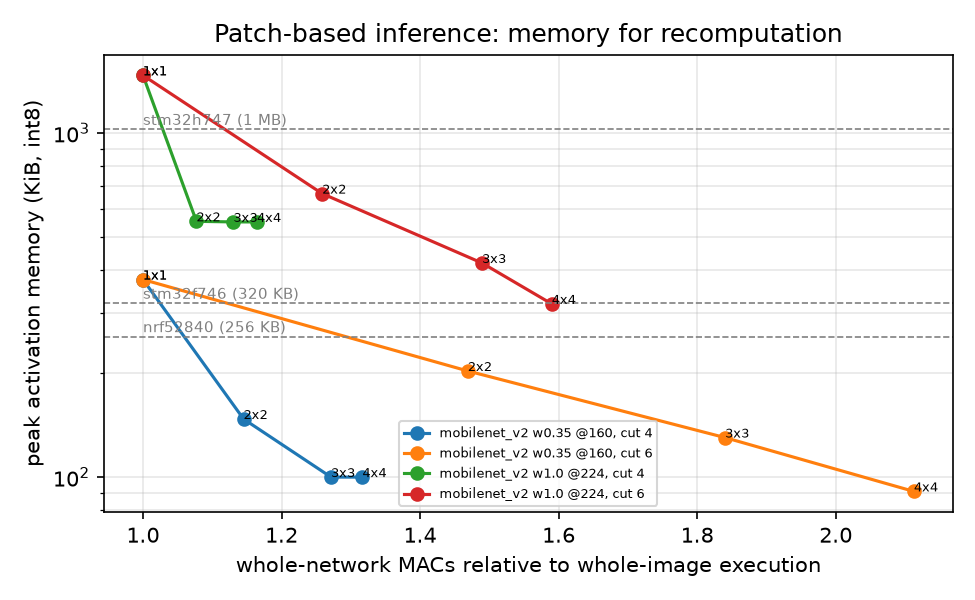
\includegraphics[width=0.85\linewidth]{patch_tradeoff.png}
\caption{按 patch 推理的权衡：横轴是整网 MACs 相对整图执行的比值，纵轴是激活峰值（KiB，对数轴）；每条线固定模型与 cut，点上标的是 $p\times p$；灰色虚线是 SRAM 预算。}\label{fig:patch}
\end{figure}

\Cref{fig:patch}的每条线从左上的 1×1（整图执行，整网开销 1.0）出发，往右下走：切得越细，峰值越低、重算越多。四条线的形状说明了两种不同的饱和：
\begin{itemize}
  \item \textbf{cut 4 的两条线（蓝、绿）先陡后平。}2×2 已经拿到大部分收益，3×3、4×4 横向右移而纵向几乎不动——峰值已经转移到 cut 之后的层（\cref{eq:e14} 的第二项），再细分只增加重算。
        绿线（1.0@224）3×3 与 4×4 重合在 564,480 B；蓝线（0.35@160）3×3 与 4×4 重合在 102,400 B。
  \item \textbf{cut 6 的两条线（橙、红）一路下降但很缓。}cut 往后移，后半段的峰值更低（0.35@160 只有 83,200 B），所以峰值仍由 patch 段决定、随 $p$ 持续下降；
        代价是每一步都要付出更多重算，橙线 4×4 的整网开销达到 2.11 倍，红线 4×4 为 1.59 倍。
\end{itemize}
与预算线对照：0.35@160 的 cut 4 在 2×2（151,040 B，整网 1.15 倍）就进入 nRF52840 的 256 KB 线以下，是这张图上进入 256 KB 最便宜的点；
1.0@224 的 cut 6、4×4 是 326,144 B，比 STM32F746 的 327,680 B 只低 1,536 B，红线最右端的点正好压在 320 KB 线上。

\begin{table}[H]
\centering\small
\caption{按 patch 推理（\texttt{patch.csv}；$p=1$ 的行即整图峰值，略去）。“面积比”$=p^2 t_\text{in}^2/\text{res}^2$，$f$ 是 stage 占整网 MACs 的比例，二者由表中数字推出}\label{tab:patch}
\setlength{\tabcolsep}{4pt}
\begin{tabular}{lrrrrrrrrr}
\toprule
模型 & cut & $p$ & $t_\text{in}$ & stage 输出 B & patch 段峰值 & 其余层峰值 & \textbf{峰值} B & stage 开销 & 整网开销 \\
\midrule
0.35@160 & 2 & 2 & 85 & 51,200 & 110,368 & 384,000 & 384,000 & 1.16 & 1.02 \\
 & 2 & 4 & 45 & 51,200 & 68,128 & 384,000 & 384,000 & 1.32 & 1.05 \\
 & 4 & 2 & 95 & 12,800 & 151,040 & 102,400 & \textbf{151,040} & 1.44 & 1.15 \\
 & 4 & 3 & 71 & 12,800 & 90,560 & 102,400 & \textbf{102,400} & 1.82 & 1.27 \\
 & 4 & 4 & 55 & 12,800 & 59,840 & 102,400 & 102,400 & 1.96 & 1.32 \\
 & 6 & 2 & 115 & 6,400 & 208,240 & 83,200 & 208,240 & 2.13 & 1.47 \\
 & 6 & 3 & 91 & 6,400 & 133,360 & 83,200 & 133,360 & 3.02 & 1.84 \\
 & 6 & 4 & 75 & 6,400 & 93,040 & 83,200 & \textbf{93,040} & 3.67 & 2.11 \\
 & 8 & 2 & 139 & 2,400 & 296,400 & 44,800 & 296,400 & 3.12 & 2.05 \\
 & 8 & 3 & 123 & 2,400 & 233,040 & 44,800 & 233,040 & 5.51 & 3.24 \\
 & 8 & 4 & 107 & 2,400 & 177,360 & 44,800 & 177,360 & 7.45 & 4.21 \\
\midrule
1.0@224 & 2 & 2 & 117 & 200,704 & 423,488 & 1,505,280 & 1,505,280 & 1.11 & 1.01 \\
 & 2 & 4 & 61 & 200,704 & 262,208 & 1,505,280 & 1,505,280 & 1.23 & 1.02 \\
 & 4 & 2 & 127 & 75,264 & 566,784 & 564,480 & \textbf{566,784} & 1.31 & 1.08 \\
 & 4 & 3 & 91 & 75,264 & 329,184 & 564,480 & 564,480 & 1.52 & 1.13 \\
 & 4 & 4 & 71 & 75,264 & 230,784 & 564,480 & 564,480 & 1.65 & 1.16 \\
 & 6 & 2 & 147 & 25,088 & 682,208 & 326,144 & 682,208 & 1.76 & 1.26 \\
 & 6 & 3 & 115 & 25,088 & 428,768 & 326,144 & 428,768 & 2.44 & 1.49 \\
 & 6 & 4 & 91 & 25,088 & 279,008 & 326,144 & \textbf{326,144} & 2.74 & 1.59 \\
 & 8 & 2 & 171 & 12,544 & 900,064 & 263,424 & 900,064 & 2.39 & 1.56 \\
 & 8 & 3 & 139 & 12,544 & 600,544 & 263,424 & 600,544 & 3.57 & 2.03 \\
 & 8 & 4 & 123 & 12,544 & 473,824 & 263,424 & 473,824 & 4.99 & 2.60 \\
\bottomrule
\end{tabular}
\end{table}

（cut 2、$p=3$ 两行与 $p=2,4$ 同理，峰值不变，见 \texttt{patch.csv}。）\Cref{tab:patch}可以按\cref{eq:e14}的两项逐行读：

\textbf{cut 2 时峰值完全不变。}0.35@160 的其余层峰值 384,000 B 就是整图峰值——峰值在 block 2（\cref{tab:profile} 第 5 步），而 cut 2 只覆盖 stem 与 block 1，峰值根本不在 patch 段里。
1.0@224 同理。切 patch 之前必须先看峰值在哪一层。

\textbf{cut 4 时峰值被“其余层”封顶。}0.35@160 从 3×3 起 patch 段峰值（90,560）已低于其余层（102,400），峰值就停在 102,400 B；
4×4 把 patch 段压到 59,840 却多付了整网 0.05 倍 MACs，什么也没换来。1.0@224 在 2×2 时两项几乎相等（566,784 对 564,480），所以 2×2 就是这条线的拐点。

\textbf{halo 随层深线性外扩。}以 0.35@160 的 4×4 为例，cut 4 / 6 / 8 处的空间下采样分别是 8 / 16 / 32 倍，tile 输出宽 5 / 3 / 2，
若没有 halo 只需输入宽 40 / 48 / 64，实际 $t_\text{in}$ 是 55 / 75 / 107，多出 15 / 27 / 43 像素。每多一层 3×3 卷积，\cref{eq:e12} 就在回推时多加一圈，
而 stride 让后面层的一圈对应输入上的若干像素。

\textbf{重算按 $p^2$ 乘以 tile 面积增长，stage 开销≈面积比。}stage 开销与“面积比”$p^2 t_\text{in}^2/\text{res}^2$ 非常接近（由表中数字算：0.35@160 cut 8、$p=4$ 面积比 7.16，stage 开销 7.45；1.0@224 cut 4、$p=2$ 面积比 1.29，stage 开销 1.31），
stage 开销总是略高于面积比，差值来自哪几层本实验没有逐层拆解。当 $t_\text{in}$ 被 halo 撑到接近全图（cut 8 的 107/160、123/224），$p^2$ 几乎就是开销倍数。

\textbf{整网口径要乘 stage 的 MACs 占比。}由 整网开销 $= 1 + (\text{stage 开销}-1)f$ 反推：1.0@224 cut 4 时 $f\approx0.25$，所以 stage 1.31 倍只对应整网 1.08 倍；
0.35@160 cut 8 时 $f\approx0.50$，stage 7.45 倍对应整网 4.21 倍。只报 stage 口径会把 1.0@224 cut 4 的代价夸大四倍，只报整网口径又会掩盖 cut 8 时前半段已经在重复算七遍。

\textbf{切得越深越细不一定更省内存。}0.35@160 cut 8、4×4 峰值 177,360 B，整网 4.21 倍；cut 4、3×3 峰值 102,400 B，整网只要 1.27 倍——前者在两个维度上都更差。
原因是 cut 8 的 tile 输入被 halo 撑到 107×107，单 tile 在 stage 内的峰值本身就很大。1.0@224 也一样：cut 8、4×4 的 473,824 B 高于 cut 6、4×4 的 326,144 B。
MCUNetV2 的做法是用 receptive field 重新设计前几层、减小 halo；本实验没有改网络。

\begin{findingbox}[：patch 推理]
（1）0.35@160 cut 4、3×3：峰值 384,000 → 102,400 B（3.75 倍），整网 MACs 多 27\%；1.0@224 cut 4、2×2：1,505,280 → 566,784 B（2.66 倍），整网 MACs 只多 7.7\%。
（2）峰值一旦转移到 cut 之后的层，再细分只增加重算；cut 越深，halo 越大，cut 8 在峰值与重算上都劣于 cut 4 / 6。
（3）重算必须同时报 stage 与整网两种口径，二者之比由 stage 的 MACs 占比 $f$ 决定（本表 $f$ 在 0.07--0.50 之间）。
\end{findingbox}

\begin{iqbox}{patch 推理为什么 $p$ 再大峰值就不降了？要继续降该怎么办？}
\cref{eq:e14} 的峰值是两项取大：patch 段（stage 输出整块 + 单 tile 峰值）和 cut 之后的其余层。$p$ 增大只压第一项；
MBv2-1.0@224 cut 4 在 $p=2$ 时两项已经相等（566,784 对 564,480），之后峰值停在 564,480。要继续降只能把 cut 后移：cut 6、4×4 降到 326,144 B，整网 1.59 倍。
但 cut 不能无限后移：cut 8 时 halo 把 tile 输入撑到 123/224，单 tile 峰值变大，4×4 反而是 473,824 B。真正的解法是 MCUNetV2 的联合设计——缩小前几层的感受野，让 halo 变小，再配合 TinyNAS 搜结构。
\end{iqbox}

\begin{iqbox}{patch 推理的代价只有多出来的 MACs 吗？}
不止。第一，cut 处的 stage 输出必须整块驻留（1.0@224 cut 4 是 75,264 B），这一项不随 $p$ 下降。
第二，MACs 开销不等于延迟开销：tile 更小，每个算子的调用与调度开销按 $p^2$ 倍增加，halo 造成不规则访存；在有 DMA 的芯片上 tile 太小会让搬运开销盖过重算（M07）。
第三，本实验只给 MACs 比值，没有测延迟；要回答“慢多少”得在板子上测。
\end{iqbox}

\section{讨论：和训练侧重计算的对照}\label{sec:discussion}
patch 推理与训练里的激活重计算（rematerialization / gradient checkpointing，mlsys-infra M14）是同一类“算力换内存”，切的维度不同：
训练是在\emph{时间}维上切——前向丢弃中间激活、反向时重算，$\sqrt{n}$ 检查点用约一次额外前向换 $O(\sqrt{n})$ 的激活内存；
推理 patch 是在\emph{空间}维上切——前几层的大激活不整块存在，代价是 tile 之间的 halo 重算。
两者的共同前提是先找到峰值在哪：训练侧看每层保存给反向的激活，推理侧看\cref{fig:profile}这样的存活曲线。
本实验的 cut 2 结果（峰值不在 patch 段，切了也白切）在训练侧的对应物是“检查点放在不是峰值的层上”。

静态内存规划在 ML 编译器里是图级 pass 之一（mlsys-infra M10）：前面的融合 pass 决定了哪些节点是别名（\cref{sec:method}），后面的规划 pass 才谈得上下界。
这也解释了为什么“忘记别名”会让峰值虚增一倍以上——规划器本身再好，也补救不了前面的 pass 没把 BN、ReLU 融掉。

\section{结论}

\begin{findingbox}[：四句话]
\begin{enumerate}
  \item 激活 arena 的下界由存活期决定（\cref{eq:e10}），MBv2-1.0@224 int8 是 1,505,280 B，每块独占要 4.68 倍。
  \item 按大小降序贪心（TFLM 默认）在 11 个配置上贴住下界；按出生顺序 first-fit 在 MobileNetV2 上恒多 13.3\%。省内存要改下界，不要换规划器。
  \item 原地 depthwise 在 MBv2 上只省 6.7\%，因为峰值移到同 block 的 expand 处；micro 网络省 30.8\%，但原地后贪心离新下界多 12.5\%。
  \item patch 推理在峰值所在的前 4 个 block 上最划算（1.0@224 用 7.7\% 整网 MACs 换 2.66 倍峰值下降）；切得更深更细，重算按 $p^2$ 涨而峰值不降。
\end{enumerate}
\end{findingbox}

\subsection*{20 秒讲法}
MCU 上先放不下的是激活峰值，不是参数。我用 torch.fx 把 MobileNetV2 的每个 int8 激活的生死区间 trace 出来，算出存活下界：1.0@224 是 1.5 MB；
TFLM 默认的按大小贪心在 11 个配置上正好等于下界，first-fit 多 13.3\%，所以要省内存只能改下界。
原地 depthwise 只省 6.7\%，因为峰值会移到同一 block 的 expand 处；按 patch 执行前 4 个 block，2×2 就把峰值压到 567 KB，整网 MACs 只多 7.7\%，但切得更深更细，重算按 $p^2$ 涨而峰值不再降。

\section{不能推出的结论}\label{sec:caveat}

\begin{caveatbox}
\begin{itemize}
  \item 只算激活，没有算 TFLM 的 interpreter 开销、im2col 等算子临时缓冲、栈与持久缓冲；真实 arena 会更大。\cref{tab:fits} 的“放得进”只针对激活，
        尤其 MBv2-1.0@96 在 nRF52840 上只余 4,096 B、1.0@224 cut 6 4×4 在 STM32F746 上只余 1,536 B，加上这些开销几乎必然放不下。
  \item MAC 开销不等于延迟开销：patch 执行时每个 tile 都更小，cache 行为与调用开销都会变；本实验没有生成代码，也没有在任何 MCU 上测延迟或内存。
  \item MCU 的 SRAM 预算是设备表里的参数，不是测量；STM32H747 的 SRAM 分布在多个域，1 MB 并不是一块连续可用的 arena。
  \item patch 实验的峰值没有叠加原地 depthwise，两种手段合用的效果本实验没有算。
  \item “按大小贪心 11/11 等于下界”是这 11 个近似链式配置上的经验结果：同一份代码在 3、3、2、2 的反例上并非最优，原地合并后 micro 网络上也多 12.5\%。
  \item torchvision 模型用随机权重，只用于形状与图结构；本报告不涉及任何精度结论，patch 推理也没有验证数值等价（只算了字节与 MACs）。
\end{itemize}
\end{caveatbox}

\section{复现}

\begin{lstlisting}[language=bash,numbers=none]
cd solutions/mit6.5940/tinyengine-memory
python -m pytest -q tests              # 9 tests
python scripts/run_experiments.py      # planners, profile, patch, summary; about 10 s
# outputs
#   artifacts/raw/planners.csv  profile_mbv2_w035_160.csv  patch.csv  summary.json
#   artifacts/figures/memory_profile.png  arena_layout.png  patch_tradeoff.png
\end{lstlisting}

脚本依赖 \texttt{torch}、\texttt{torchvision}、\texttt{matplotlib}，并从 \texttt{../lab2-quantization/code} 导入 micro 网络、从仓库根目录导入 \texttt{edge\_harness} 设备表。
全部计算在 CPU 上完成（\texttt{torch.set\_num\_threads(2)}），不需要 GPU 或开发板。

\begin{thebibliography}{99}
\bibitem{mcunet} J.~Lin, W.-M.~Chen, Y.~Lin, J.~Cohn, C.~Gan, S.~Han. MCUNet: Tiny Deep Learning on IoT Devices. \emph{NeurIPS}, 2020.
\bibitem{mcunetv2} J.~Lin, W.-M.~Chen, H.~Cai, C.~Gan, S.~Han. MCUNetV2: Memory-Efficient Patch-based Inference for Tiny Deep Learning. \emph{NeurIPS}, 2021.
\bibitem{mobilenetv2} M.~Sandler, A.~Howard, M.~Zhu, A.~Zhmoginov, L.-C.~Chen. MobileNetV2: Inverted Residuals and Linear Bottlenecks. \emph{CVPR}, 2018.
\bibitem{chen2016} T.~Chen, B.~Xu, C.~Zhang, C.~Guestrin. Training Deep Nets with Sublinear Memory Cost. arXiv:1604.06174, 2016.
\end{thebibliography}

\end{document}
